% eRisk 2026 Task 1 — Architecture (readable TikZ)
% Compile: export PATH="/Library/TeX/texbin:$PATH" && pdflatex architecture_erisk2026.tex

\documentclass[11pt]{article}
\usepackage{tikz}
\usepackage{graphicx}
\usepackage[margin=0.75in]{geometry}
\pagestyle{empty}

\usetikzlibrary{positioning, arrows.meta, fit, backgrounds, calc}

% --- Readable sizes (no global resizebox — that was making everything microscopic) ---
\definecolor{llmfill}{HTML}{E8F4FC}
\definecolor{llmframe}{HTML}{2980B9}
\definecolor{rulefill}{HTML}{F0F3F4}
\definecolor{ruleframe}{HTML}{566573}
\definecolor{patfill}{HTML}{D5F5E3}
\definecolor{patframe}{HTML}{1E8449}
\definecolor{knowfill}{HTML}{FCF3CF}
\definecolor{knowframe}{HTML}{B7950B}
\definecolor{outfill}{HTML}{EBDEF0}
\definecolor{outframe}{HTML}{7D3C98}

\newcommand{\boxfont}{\sffamily}

\tikzset{
  bigbox/.style={
    draw,
    rounded corners=3pt,
    align=center,
    inner sep=8pt,
    minimum width=3.8cm,
    font=\boxfont
  },
  llm/.style={bigbox, fill=llmfill, draw=llmframe, line width=0.9pt},
  rule/.style={bigbox, fill=rulefill, draw=ruleframe, line width=0.9pt},
  pat/.style={bigbox, fill=patfill, draw=patframe, line width=0.9pt},
  know/.style={bigbox, fill=knowfill, draw=knowframe, line width=0.75pt, minimum width=3.2cm, font=\small\boxfont},
  outn/.style={bigbox, fill=outfill, draw=outframe, line width=0.9pt},
  arr/.style={-{Stealth[length=3mm]}, thick, shorten >=2pt, shorten <=2pt},
  arrdash/.style={-{Stealth[length=3mm]}, thick, dashed, shorten >=2pt, shorten <=2pt},
  lbl/.style={font=\small\sffamily, inner sep=2pt}
}

\begin{document}
\thispagestyle{empty}

% ========== PAGE 1: Plain-English overview (large text) ==========
\begin{center}
{\Large\bfseries\sffamily eRisk 2026 — How the system works}\\[0.4em]
{\normalsize\sffamily\color{ruleframe}
One \textbf{doctor AI} (the \textbf{Prober}) chats with one \textbf{patient AI} (a Llama model with a persona adapter).\\
After each reply, an \textbf{Extractor} updates a depression checklist (BDI-II).\\
A \textbf{Stopper} decides when to stop chatting; then a \textbf{Scorer} outputs a total score + up to four key symptoms.}
\end{center}

\vspace{0.6em}

\begin{center}
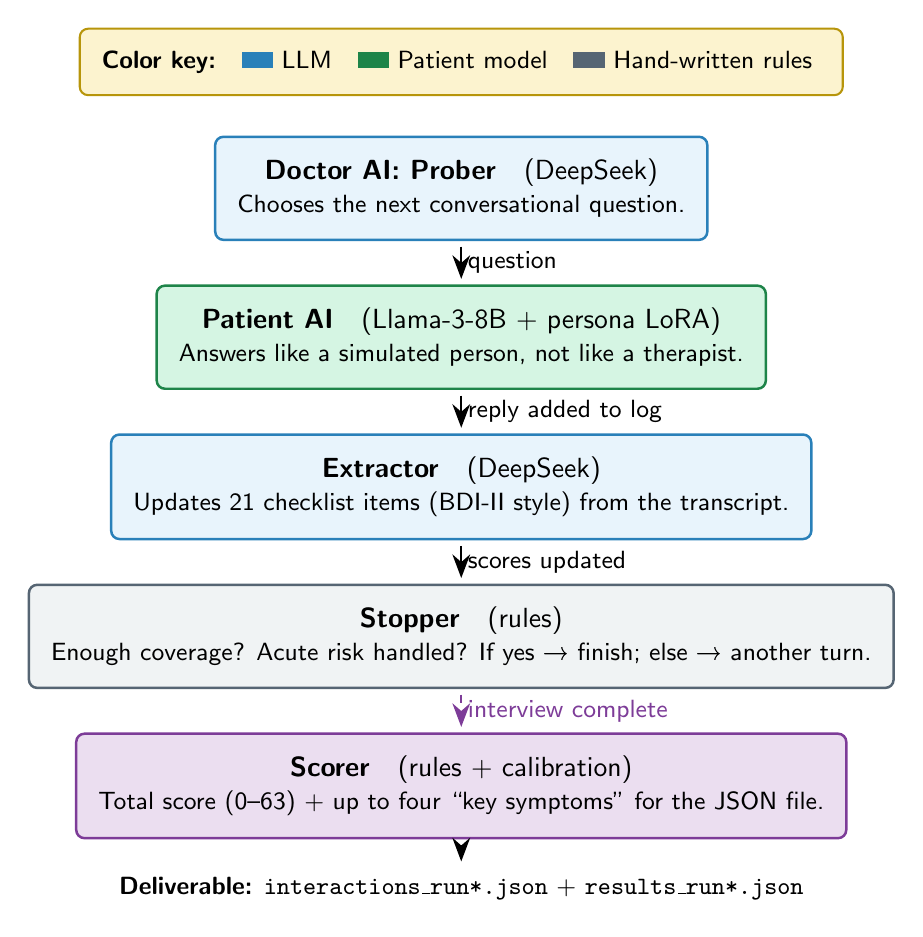
\begin{tikzpicture}[
    node distance=0.55cm,
    >={Stealth[length=3mm]}
  ]

  % Vertical flow — easiest to read top → bottom
  \node[llm, minimum height=1.25cm, minimum width=5.2cm] (p) {%
    \textbf{Doctor AI: Prober}\quad (DeepSeek)\\
    \small Chooses the next conversational question.};
  \node[pat, below=of p, minimum height=1.25cm, minimum width=5.2cm] (u) {%
    \textbf{Patient AI}\quad (Llama-3-8B + persona LoRA)\\
    \small Answers like a simulated person, not like a therapist.};
  \node[llm, below=of u, minimum height=1.25cm, minimum width=5.2cm] (e) {%
    \textbf{Extractor}\quad (DeepSeek)\\
    \small Updates 21 checklist items (BDI-II style) from the transcript.};
  \node[rule, below=of e, minimum height=1.15cm, minimum width=5.2cm] (s) {%
    \textbf{Stopper}\quad (rules)\\
    \small Enough coverage? Acute risk handled? If yes → finish; else → another turn.};
  \node[outn, below=of s, minimum height=1.15cm, minimum width=5.2cm] (sc) {%
    \textbf{Scorer}\quad (rules + calibration)\\
    \small Total score (0--63) + up to four ``key symptoms'' for the JSON file.};
  \node[below=0.35cm of sc, font=\small\boxfont] (j) {\textbf{Deliverable:} \texttt{interactions\_run*.json} + \texttt{results\_run*.json}};

  \draw[arr] (p) -- node[right, lbl] {question} (u);
  \draw[arr] (u) -- node[right, lbl] {reply added to log} (e);
  \draw[arr] (e) -- node[right, lbl] {scores updated} (s);
  \draw[arrdash, outframe] (s) -- node[right, lbl] {interview complete} (sc);
  \draw[arr] (sc) -- (j);

  \node[know, above=0.5cm of p.north, minimum width=5.4cm] (legend) {%
    \textbf{Color key:}\quad
    {\color{llmframe}\rule{0.4cm}{0.2cm}}\ LLM\quad
    {\color{patframe}\rule{0.4cm}{0.2cm}}\ Patient model\quad
    {\color{ruleframe}\rule{0.4cm}{0.2cm}}\ Hand-written rules
  };

\end{tikzpicture}
\end{center}

\vspace{0.5em}
{\small\sffamily
\textbf{Each turn (simplified):} Prober asks $\rightarrow$ Patient answers $\rightarrow$ risk features + Extractor update scores $\rightarrow$ Stopper decides ``another turn?'' or ``done.''\\
When ``done,'' the Scorer turns the running checklist into the final BDI total and key symptoms.\\
\textbf{A2A} = agent-to-agent: a doctor model and a patient model, plus separate rule/LLM steps — not one chatbot doing everything.}

\newpage

% ========== PAGE 2: Detailed pipeline (matches code; still no tiny resizebox) ==========
{\large\bfseries\sffamily Detailed pipeline (implementation)}\\[0.5em]
{\small\sffamily Same loop as \texttt{src/orchestrator.py} — read top-to-bottom, then follow the curved arrow back.}

\vspace{0.5em}

\noindent
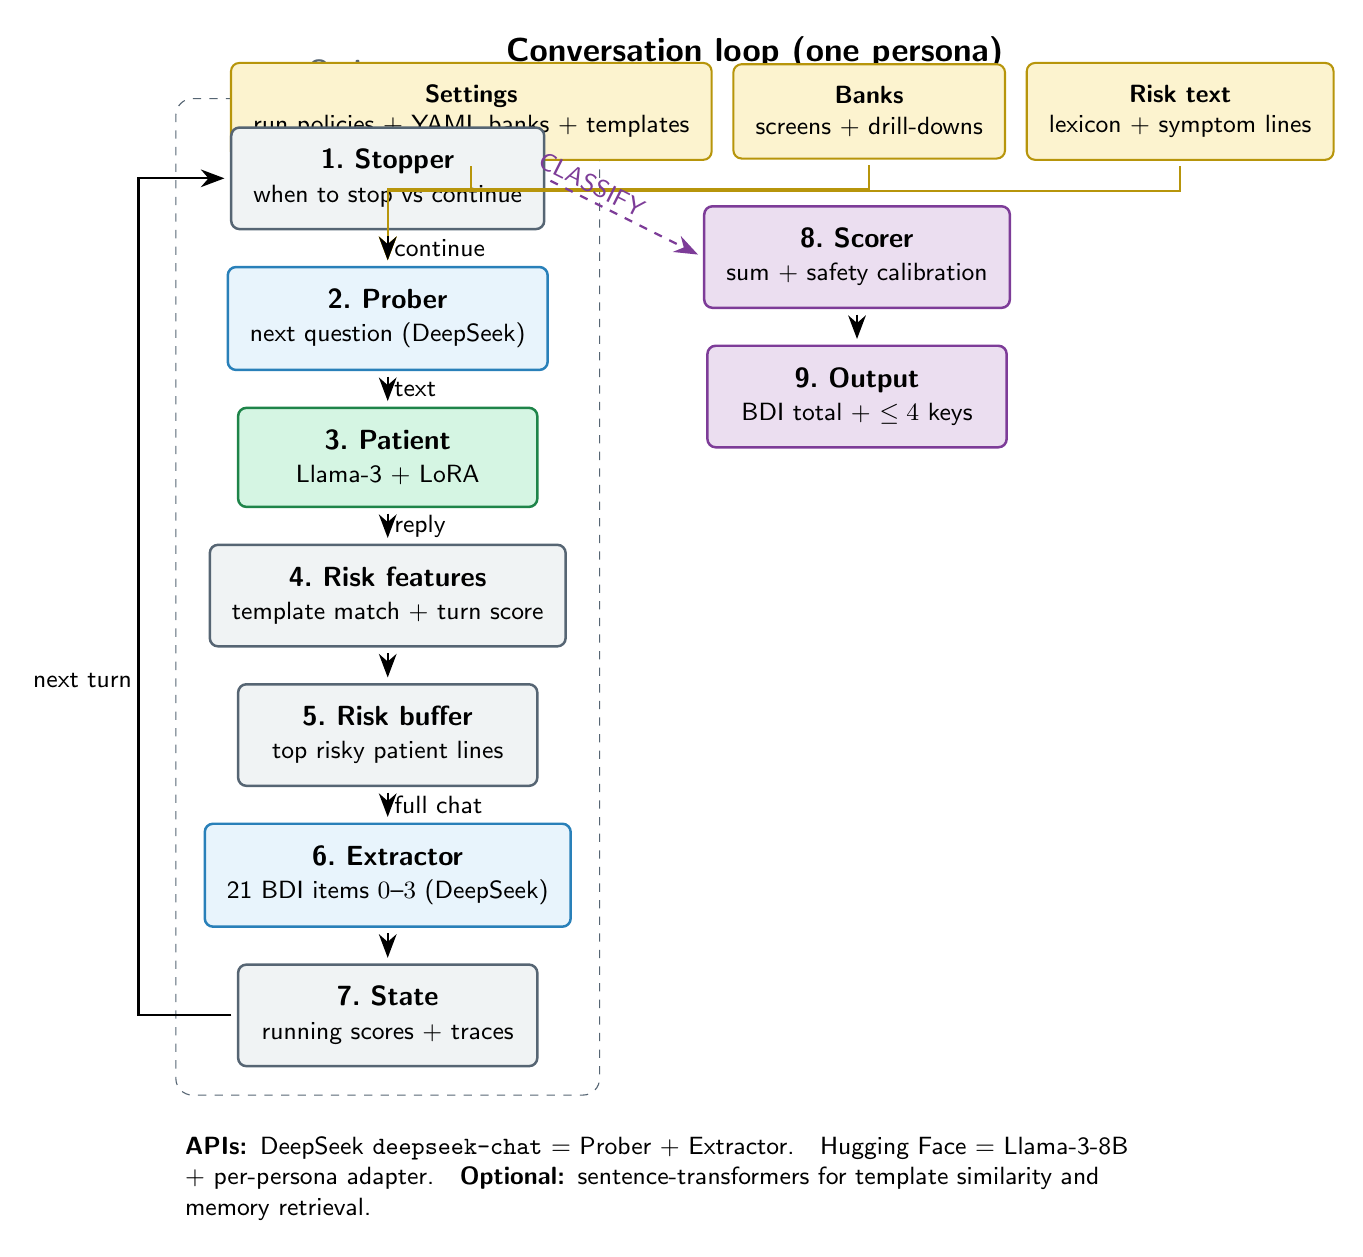
\begin{tikzpicture}[
    node distance=0.45cm,
    >={Stealth[length=2.8mm]}
  ]

  \node[font=\large\bfseries\sffamily] (title) {Conversation loop (one persona)};

  \node[know, below=0.4cm of title, anchor=center, xshift=-3.6cm] (policy) {\textbf{Settings}\\run policies + YAML banks + templates};
  \node[know, right=0.25cm of policy] (banks) {\textbf{Banks}\\screens + drill-downs};
  \node[know, right=0.25cm of banks] (templates) {\textbf{Risk text}\\lexicon + symptom lines};

  \node[rule, below=0.85cm of policy.west, anchor=west, minimum height=1.05cm] (stopper) {\textbf{1.\ Stopper}\\\small when to stop vs continue};
  \node[llm, below=of stopper, minimum height=1.05cm] (prober) {\textbf{2.\ Prober}\\\small next question (DeepSeek)};
  \node[pat, below=of prober, minimum height=1.05cm] (persona) {\textbf{3.\ Patient}\\\small Llama-3 + LoRA};
  \node[rule, below=of persona, minimum height=1.05cm] (evidence) {\textbf{4.\ Risk features}\\\small template match + turn score};
  \node[rule, below=of evidence, minimum height=1.05cm] (buffer) {\textbf{5.\ Risk buffer}\\\small top risky patient lines};
  \node[llm, below=of buffer, minimum height=1.05cm] (extractor) {\textbf{6.\ Extractor}\\\small 21 BDI items $0$--$3$ (DeepSeek)};
  \node[rule, below=of extractor, minimum height=1.05cm] (state) {\textbf{7.\ State}\\\small running scores + traces};

  \node[outn, right=2.0cm of stopper, yshift=-1.0cm, minimum height=1.05cm] (scorer) {\textbf{8.\ Scorer}\\\small sum + safety calibration};
  \node[outn, below=of scorer, minimum height=0.95cm] (out) {\textbf{9.\ Output}\\\small BDI total + $\leq 4$ keys};

  \begin{scope}[on background layer]
    \node[
      draw=ruleframe,
      dashed,
      rounded corners=6pt,
      inner sep=10pt,
      fit={(stopper) (prober) (persona) (evidence) (buffer) (extractor) (state)},
      label={[font=\normalsize\bfseries\sffamily, yshift=3pt]above:\textcolor{ruleframe}{Orchestrator}}
    ] (orchbox) {};
  \end{scope}

  \draw[arr, knowframe] (policy.south) -- +(0,-0.38) -| (prober.north);
  \draw[arr, knowframe] (banks.south) -- +(0,-0.38) -| (prober.north);
  \draw[arr, knowframe] (templates.south) -- +(0,-0.38) -| (prober.north);

  \draw[arr] (stopper) -- node[right, lbl] {continue} (prober);
  \draw[arr] (prober) -- node[right, lbl] {text} (persona);
  \draw[arr] (persona) -- node[right, lbl] {reply} (evidence);
  \draw[arr] (evidence) -- (buffer);
  \draw[arr] (buffer) -- node[right, lbl] {full chat} (extractor);
  \draw[arr] (extractor) -- (state);

  \coordinate[left=1.25cm of state.west] (looppt);
  \draw[arr] (state.west) -- (looppt) |- node[lbl, pos=0.2, left] {next turn} (stopper.west);

  \draw[arrdash, outframe] (stopper.east) -- node[lbl, above, sloped, near start] {CLASSIFY} (scorer.west);
  \draw[arr] (scorer) -- (out);

  \node[anchor=north west, align=left, font=\small\sffamily, text width=\textwidth] at ($(orchbox.south west)+(0,-0.4)$) {%
    \textbf{APIs:} DeepSeek \texttt{deepseek-chat} = Prober + Extractor.\quad
    Hugging Face = Llama-3-8B + per-persona adapter.\quad
    \textbf{Optional:} sentence-transformers for template similarity and memory retrieval.%
  };

\end{tikzpicture}

\end{document}
